\documentclass{scrartcl}

\usepackage{helvet}
\usepackage[T1]{fontenc}
\usepackage[ngerman]{babel}
\usepackage[utf8]{inputenc}
\usepackage{enumitem}
\usepackage{hyperref}
\usepackage{graphicx}
\renewcommand{\familydefault}{\sfdefault}
%----------------------------------
% thomi fa list implementation
%----------------------------------

\newlist{falist}{enumerate}{2}
\setlist[falist,1]{label={/FA\arabic{falisti}\arabic{falistii}/},align=left,labelwidth=17pt,labelsep=3pt,leftmargin=20pt}
\setlist[falist,2]{label={/FA\arabic{falisti}\arabic{falistii}/}}%,align=left,labelwidth=17pt,labelsep=3pt,leftmargin=0pt}

\usepackage{chngcntr}
\counterwithin{falistii}{falisti}

\newlist{pdlist}{enumerate}{2}
\setlist[pdlist,1]{label={/PD\arabic{pdlisti}\arabic{pdlistii}/},align=left,labelwidth=17pt,labelsep=3pt,leftmargin=20pt}
\setlist[pdlist,2]{label={/PD\arabic{pdlisti}\arabic{pdlistii}/}}%,align=left,labelwidth=17pt,labelsep=3pt,leftmargin=0pt}
\counterwithin{pdlistii}{pdlisti}

\newlist{nflist}{enumerate}{2}
\setlist[nflist,1]{label={/NF\arabic{nflisti}\arabic{nflistii}/},align=left,labelwidth=17pt,labelsep=3pt,leftmargin=20pt}
\setlist[nflist,2]{label={/NF\arabic{nflisti}\arabic{nflistii}/}}%,align=left,labelwidth=17pt,labelsep=3pt,leftmargin=0pt}
\counterwithin{nflistii}{nflisti}

\newlist{telist}{enumerate}{2}
\setlist[telist,1]{label={/T\arabic{telisti}\arabic{telistii}/},align=left,labelwidth=17pt,labelsep=3pt,leftmargin=20pt}
\setlist[telist,2]{label={/T\arabic{telisti}\arabic{telistii}/}}%,align=left,labelwidth=17pt,labelsep=3pt,leftmargin=0pt}
\counterwithin{telistii}{telisti}

\begin{document}

\begin{titlepage}

\title{Pflichtenheft: Lambda - Das Spiel, Team Dirty Bit Misses}
\author{Luca Becker, Henrike Hardt, Larissa Schmid, Adrian Schulte, Maik Wiesner}
\date{\today}

\maketitle
\thispagestyle{empty}

\end{titlepage}

\clearpage

\tableofcontents
\thispagestyle{empty}

\clearpage
\setcounter{page}{1}

\section{Einleitung}

Der derzeitige und auch kommende Ingenieursmangel in Deutschland ist
schon seit Langem Thema in den Medien. „Auf jeden Bewerber kommen
etwa 4 freie Stellen“%
\footnote{http://www.ingenieurwesen-studieeren.de/ingenieurmangel/%
}, „jeder zweite angehende Ingenieur bricht sein Studium ab“%
\footnote{http://www.zeit.de/studium/hochschule/2013-10/ingenieure-unis-fachkraeftemangel%
}, all diese Nachrichten geben Grund zur Sorge in Hinblick auf Deutschland
als Technologiestandort. Unsere Volkswirtschaft beruht nicht mehr
auf Wertschöpfung aus dem ersten und zweiten, sondern vor allem aus
dem dritten Sektor – damit dies weiterhin funktionieren kann, werden
vor allem Ingenieure benötigt. Doch an dem derzeitigen Mangel ist
nicht nur die Überalterung unserer Gesellschaft schuld, sondern vor
allem auch die fehlende Begeisterung von Jugendlichen für die sogenannten
MINT-Fächer (Mathematik, Informatik, Naturwissenschaft, Technik).
Um Deutschland als Standort auch weiterhin wettbewerbsfähig zu halten,
ist es somit wichtig, Kinder schon frühestmöglich spielerisch an Fragestellungen
aus diesen Bereichen heranzuführen. 

In der Informatik ist der Lambda-Kalkül ein wichtiges Konstrukt, der
zum Beispiel die Entwicklung funktionaler Programmiersprachen wesentlich
beeinflusst hat. Obwohl er damit eine große Bedeutung hat und sehr
mächtig ist in Bezug auf sowohl die Theoretische Informatik als auch
funktionale Programmierung, so sind die grundlegenden Regeln dennoch
nicht allzu komplex und leicht verständlich. 

Um Kindern also schon im Grundschulalter eine erste Auseinandersetzung
mit Themen der Informatik und damit auch der Ingenieurswissenschaften
zu bieten, eignet sich der Kalkül also sehr gut. Unsere nachfolgend
dargelegte Visualisierung der Funktionsweise des Kalküls mithilfe
von einfachen Formen und sie ineinander umwandelnden Maschinen ist
dabei besonders kindgerecht, wodurch der Kalkül anhand von einfachen
Lambda-Ausdrücken einfacher verstanden und verinnerlicht werden kann.
Diese Idee soll nun als Android-App umgesetzt werden, sodass Kinder
selbständig spielen können, der Fortschritt im Spiel aber auch jederzeit
durch Eltern oder Lehrkräfte einsehbar ist. 

\clearpage

\section{Zielbestimmungen}


Die Kinder sollen durch das Spiel in die Lage versetzt werden, sich die Prinzipien des Lambda Kalküls spielerisch zu erarbeiten ohne über Vorkenntnisse zu verfügen.

\subsection{Musskritieren}

\begin{enumerate}
	\item Spielerisches Vermitteln des Lambda Kalküls für Kinder ab acht Jahren
	\item Das Spiel muss in der Simulationsumgebung von Android laufen
	\item komplett über das simulierte Touchinterface bedienbar sein
	\item eine modulare Architektur besitzen (z.B. Model-View-Controller-Prinzip)
	\item mindestens fünf individuelle Level
	\item Tutorial Level
\end{enumerate}

\subsection{Wunschkriterien}

\begin{enumerate}
	\item \label{wunsch:werkstatt}Werkstatt zum Umbauen von Maschinen
	\item \label{wunsch:highscore}Highscore-Tabelle
	\item \label{wunsch:challengemode}Challengemode mit Zeitdruck
	\item \label{wunsch:multilang}Auslieferung in mehreren Sprachen
	\item \label{wunsch:8bit}8-Bit Grafik
	\item \label{wunsch:multiplechar}Mehrere Spielcharaktere (männlich, weiblich)
	\item \label{wunsch:multiplemode}Mehrere Spielmodi (siehe Aufgabentyp \ref{aufgabentyp:fehlerfindung})
    \item \label{wunsch:story} Begleitende Story
\end{enumerate}

\subsection{Abgrenzungskritieren}

\begin{enumerate}
	\item Kein Onlinemodus
	\item Kein Multiplayer Modus
	\item Keine vorgesehene Kompatiblität mit anderen Geräten/Betriebssystem ohne Emulation
\end{enumerate}

\clearpage

\section{Spielaufbau}

Das Spiel besteht aus einem Jump 'n' Run und einem Rätselteil, die in einer engen Verbindung zueinander stehen. Der Jump 'n' Run Teil dient dazu die benötigten Bauteile für den Rätselteil zu sammeln. Im Rätselteil werden die Bauteile zusammengesetzt, was wiederrum das nächste Level freischaltet.

\subsection{Spielprinzip}

\subsection{Spielelemente}

Zu Beginn eines Levels wird die Spielerfigur angezeigt und bewegt zweidimensional durch die Welt und wird vom Spieler gesteuert.

\begin{description}
	\item[Spielerfigur] bewegt sich durch die Welt, sammelt Gegenstände um mit diesen die Levelquest zu lösen
	\item[Spielwelt] zweidimensionale Spielwelt auf einem Raster basierend, in der sich der Spieler im Jump 'n' Run Teil bewegt
	\item[Collectable Items] \label{elemente:collectable}sind in der Spielwelt verteilt und müssen von der Spielfigur eingesammelt werden um im Rätselteil eingesetzt zu werden. Diese bestehen aus:
	\begin{enumerate}[label=\arabic*]
		\item Maschinen (entspricht der Abstraktion)
		\item Metallstücke (entspricht der Variablen)
		\item Maschinen-Cluster (entspricht der Applikation)
	\end{enumerate}
	\item[Levelquest] sind gegebene Aufgaben die zum Abschließen des Levels erfüllt werden müssen
	\item[Leveltür] bildet den Abschluss eines Levels. Sobald alle Quests in dem Level gelöst wurden wird die Tür freigeschaltet
\end{description}

\subsection{Regeln}

\subsection{Aufgabentypen}

\begin{enumerate}
	\item \label{aufgabentyp:puzzle}
	\item \label{aufgabentyp:fehlerfindung}
\end{enumerate}

\clearpage

\section{Produkteinsatz}

Das Produkt soll auf jedem Android Gerät ab Android 4.0 einsatzfähig sein. Ein Einsatz auf Emulatoren der Android Plattform ist ebenfalls vorgesehen.

\subsection{Anwendungsbereich}

\begin{enumerate}
	\item Einsatz an Grundschulen, die das Programm zur Vermittlung von Wissen nutzen
	\item Freizeitgestaltung von unter zwölfjährigen Kindern
\end{enumerate}

\subsection{Zielgruppen}

Die Zielgruppe besteht überwiegend aus Kinder im Alter von acht bis zwölf Jahren, die das Spiel entweder aus Interesse oder aber das Spiel im Rahmen eines Projektes an der Schule spielen.

\subsection{Betriebsbedingungen}

Der primäre Einsatzbereich 

\clearpage

\section{Produktumgebung}

\clearpage

\section{Funktionale Anforderungen}

\begin{falist}
	\item Tutorial Modus findet nach dem ersten Starten des Spiels statt
	\begin{falist}
        \item Der Tutorial Modus basiert auf einem minimum an textuellen Erklärungen
        \item Erklärt die Funktionsweise des Spiels
		\item Ein wiederholtes Starten des Tutorial Modus ist möglich
	\end{falist}
	\item Spielerprofile
	\begin{falist}
		\item Anlegen von Spielerprofilen
		\item Bearbeiten von Spielerprofilen
		\item Löschen von Spielerprofilen
		\item Wechseln zu Spielerprofilen
	\end{falist}
	\item Levelmenü bietet eine Auswahl der freigeschalteten Level
    \begin{falist}
        \item Das erste Level ist automatisch freigeschaltet
    \end{falist}
	\item Spieleinstellungen
	\begin{falist}
		\item Einstellen der Lautstärke
		\item An/Aus für Lautstärke
	\end{falist}
	\item Spielestatistiken
	\begin{falist}
		\item
	\end{falist}
	\item Interaktion mit den Spielelementen aus Nr. \ref{elemente:collectable}
	\begin{falist}
		\item Aufnehmen von Spielelementen
		\item Abgabe für die Levelquests
	\end{falist}
	\item Hinweise
	\item Infobereich
    \item Achievements
\end{falist}

\clearpage

% ---------------
% Produktdaten
% ---------------
\section{Produktdaten}
Das Produkt muss Daten speichern und verwalten, insbesondere: 

\subsection{Profildaten}

\begin{pdlist}
    \item Profile, bestehend aus 
    \begin{pdlist}
        \item Name des Spielers
        \item Avatar
        \item profilbezogene Einstellungen(Hintergrund, Musik etc.) 
        \item profilbezogener Spielfortschritt(gelöste Level, Achievements, etc.)
    \end{pdlist}
    \item Spielstatistiken
    \begin{pdlist}
        \item Spieldauer
        \item Anzahl gelöste Level
        \item Anzahl Achievments
        \item Anzahl Niederlagen/Versagen/Looser sein/Noob/Deine mudda alda
    \end{pdlist}
\end{pdlist}

\subsection{Einstellungen}

\clearpage

% ---------------
% Nichtfunktionale Anforderungen
% ---------------

\section{Nichtfunktionale Anforderungen}

\subsection{Allgemeine Ziele}

\begin{nflist}
    \item
\end{nflist}

\subsection{Benutzbarkeit, Performance, Stabilität}
\begin{nflist}[resume]
	\item Das Starten eines Levels beträgt höchstens 10s 
	\item Das Programm läuft stabil: 
	\begin{nflist}
		\item Es treten keine Abstürze der Software auf 
		\item Ladezeiten befinden sich in einem akzeptablen Rahmen. 
	\end{nflist}
	\item Die Auswertung eines Levels(Sieg oder Niederlage) dauert max. 5 Sekunden. 
	\item mind. 75\% Testüberdeckung 
	\item Es wird nur die Berechtigung für den Speicherzugriff(Lesen
	und Schreiben) benötigt. 
	\item Der benötigte Speicherverbrauch reduziert sich auf ein Minimum. 
	\item Nach Beendigung eines Levels wird der Spielstand automatisch gespeichert.
\end{nflist}

\subsection{Qualität und Rechtliches}

\begin{nflist}[resume]
	\item Das Programm verwendet für Dateien folgende Standards: 
	\begin{itemize}
		\item WAV, OGG für Audio Dateien 
		\item SVG für Vektorgrafiken 
		\item PNG, JPG für pixelbasierte Grafiken 
	\end{itemize}
	\item Die Auslieferung der finalen Version erfolgt in Form einer .apk-Datei.
	\item Impressum und ausschließliche Verwendung von frei verfügbare Biblitoheken
	für den Fall der Veröffentlichung
\end{nflist}

\clearpage

% ---------------
% Systemmodelle
% ---------------
\section{Systemmodelle}

\subsection{Allgemeiner Appaufbau}

Der hier gezeigte Systemaufbau ist lediglich eine grobe "Skizze",
die die zusammenhänge zwischen den einzelnen Menüs verdeutlichen soll.
Außerdem soll es helfen die Gestaltung und Aufteilung der App zu verdeutlichen.\\
Allgemein soll jedoch beibehalten werden, das so viel wie möglich ohne Text, sondern durch Symbolik erklärt bzw. dargestellt werden soll. Da die Zielgruppe nicht zwangsläufig lesen und schreiben kann.
\begin{enumerate}
	\begin{minipage}{1\textwidth}
		\item \subsection*{Ladebildschirm:}
		Nach dem Starten der App, öffnet diese im Ladebildschirm, in diesem werden für die App notwendige Daten geladen, um zu Garantieren das das Spiel flüssig und Fehlerfrei läuft. Benutzeingaben sind zu diesem Zeitpunkt nicht möglich.\\
		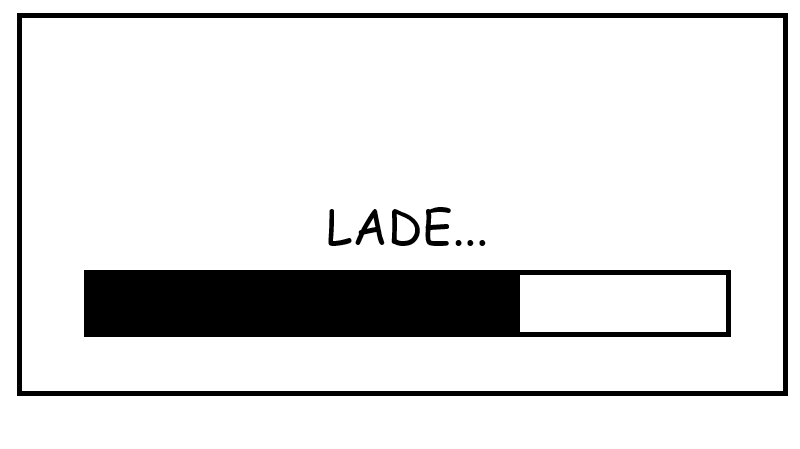
\includegraphics[width=\textwidth, height=7.5cm]{assets/LoadScreen}
	\end{minipage}
	
	\begin{minipage}{1\textwidth}
		\item \subsection*{Profilmenü:}
		Das Profilmenü öffnet sich unmittelbar nach erfolgreicher Beendigung des Ladevorgangs(Nähere informationen zum Ablauf und Ausnahmen folgen im Kapitel Szenarien).
		In diesem Menü kann der Spieler aus den bestehenden Spielerprofilen auswählen oder in das Menü zum anlegen eines neuen Spielers gelangen.\\
		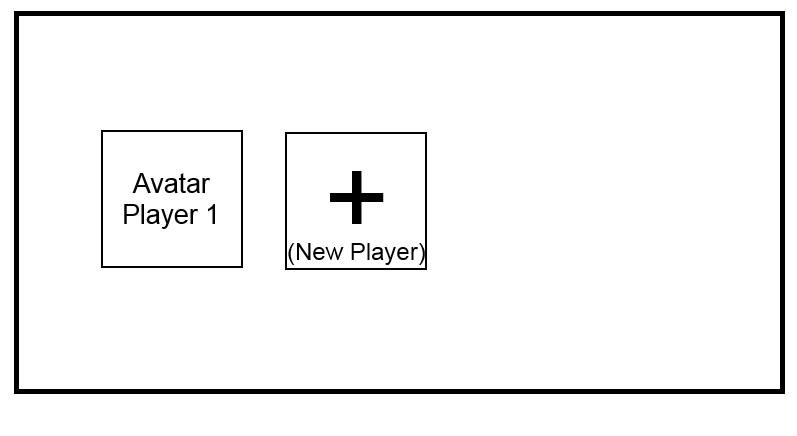
\includegraphics[width=\textwidth, height=7.5cm]{assets/PlayerScreen}
	\end{minipage}
	
	\begin{minipage}{1\textwidth}
		\item \subsection*{Profil anlegen:}
		In diesem Menü kann ein neues Spielerprofil vom Spieler angelegt werden. Der Spieler kann einen Namen für das Profil eingeben und aus einer gegebenen Menge an Avataren einen als Identifikationsmerkmal aussuchen.Sollte der Spieler hier abbrechen, so gelangt er zurück ins Profilmenü, ansonsten landet er entweder im Tutorial oder im Hauptmenü(Mehr dazu im Kapitel Szenarien)\\
		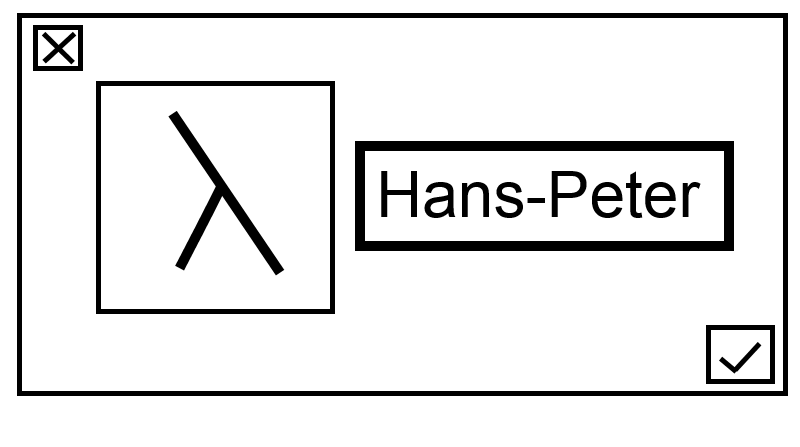
\includegraphics[width=\textwidth, height=7.5cm]{assets/CreateProfile}
	\end{minipage}
	
	\begin{minipage}{1\textwidth}
		\item \subsection*{Hauptmenü:}
		Dies ist der Zentrale Knotenpunkt der App. von hier aus kann der Spieler zur Stageauswahl, den Einstellungen, seiner Statistik, zurück ins Profilmenü gelangen oder das Spiel komplett verlassen.\\
		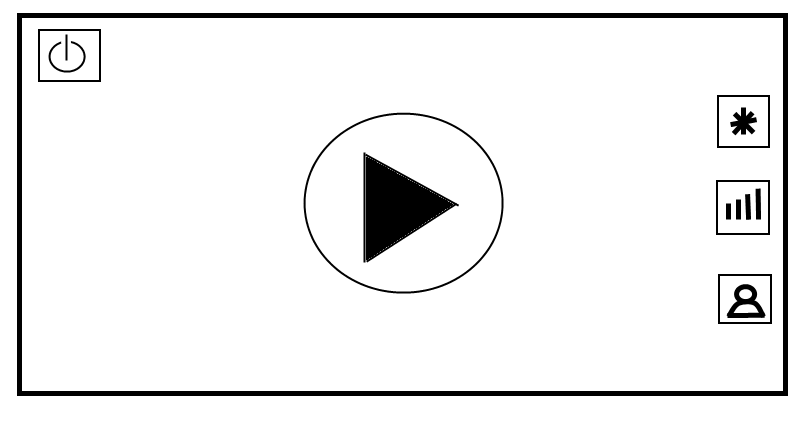
\includegraphics[width=\textwidth, height=7.5cm]{assets/Mainmenu}
	\end{minipage}
	
	\begin{minipage}{1\textwidth}
		\item \subsection*{Einstellungen:}
		Hier können verschiedene grundlegende Einstellungen vorgenommen werden. Außerdem gelangt man von hier ins Profilbearbeitungsmenü und zur Ansicht aller Achievments (Achievmentmenu).Der Zurück-Button führt ins Hauptmenü, beim verlassen werden sämtliche Änderungen gespeichert.\\
		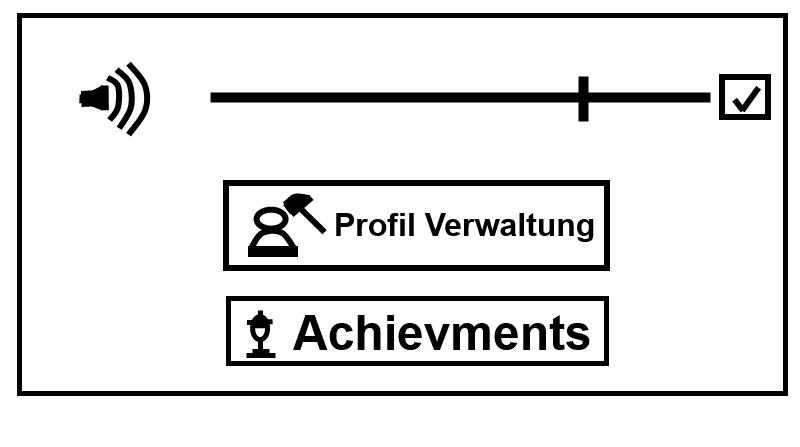
\includegraphics[width=\textwidth, height=7.5cm]{assets/Einstellungen}
	\end{minipage}

	\begin{minipage}{1\textwidth}
		\item \subsection*{Profilbearbeitungsmenü:}
		Dieses Menü ist absolut identisch mit dem Menü zum Anlegen eines neuen Spielerprofils. Der einzige Unterschied ist das jeder Weg aus diesem Menü zurück in die Einstellungen führt.\\
		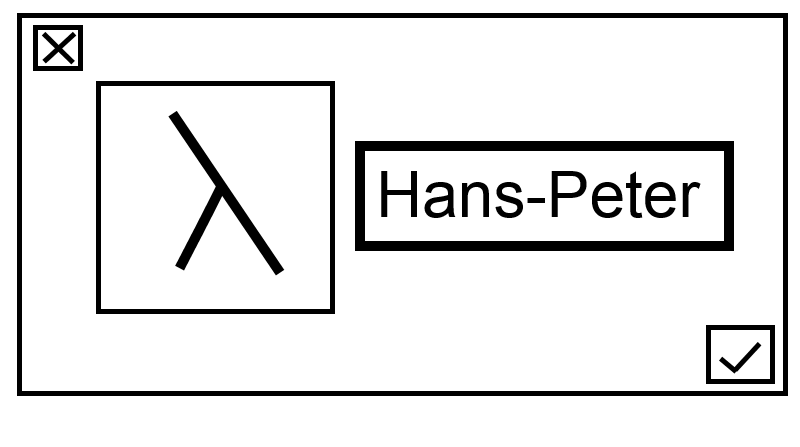
\includegraphics[width=\textwidth, height=7.5cm]{assets/CreateProfile}
	\end{minipage}

	\begin{minipage}{1\textwidth}
		\item \subsection*{Achievments:}
		Hier sind alle Achievments zu sehen, die die man schon erlangt hat sind durch ein Bild gekennzeichnet, ansonsten ist dort ein Platzhalter zu sehen. Ein Abbruch führt zurück in die Einstellungen.\\
		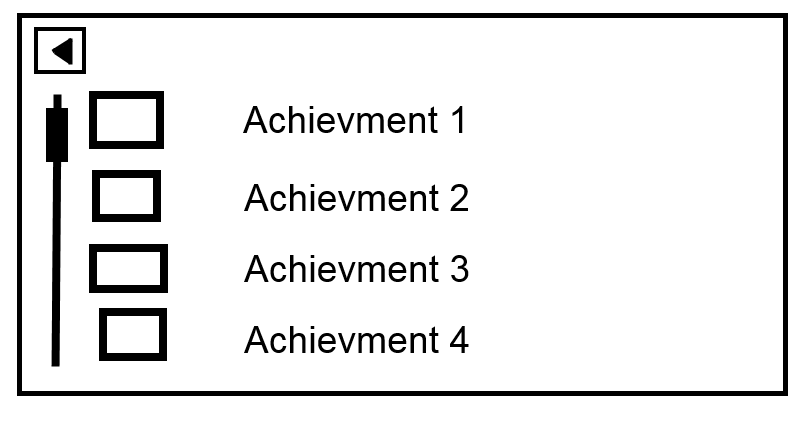
\includegraphics[width=\textwidth, height=7.5cm]{assets/Achievments}
	\end{minipage}
	
	\begin{minipage}{1\textwidth}
		\item \subsection*{Stagemenü:}
		Hier kann man sich eine Stage zum Spiele auswählen sie sind der Schwierigkeit nach geordnet und können im Spielverlauf freigeschaltet werden.\\
		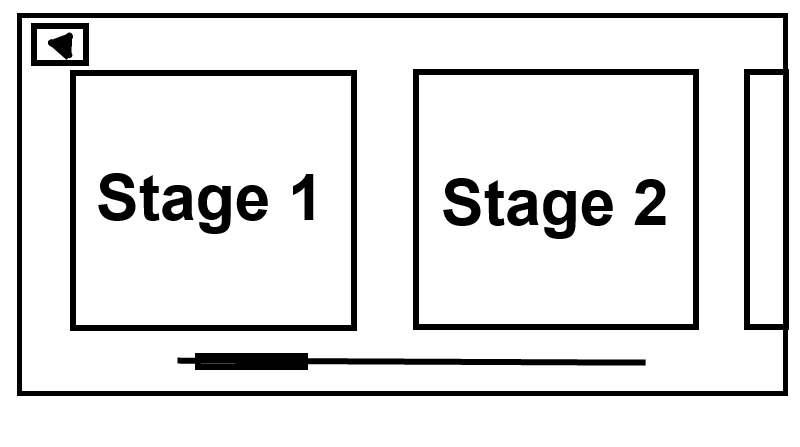
\includegraphics[width=\textwidth, height=7.5cm]{assets/Stagemenu}
	\end{minipage}
	
	\begin{minipage}{1\textwidth}
		\item \subsection*{Levelmenü:}
		hier kann ein Level der Stage in der man sich aktuell befindet gestartet werden.(auch diese müssen nach und nach freigeschaltet werden).\\
		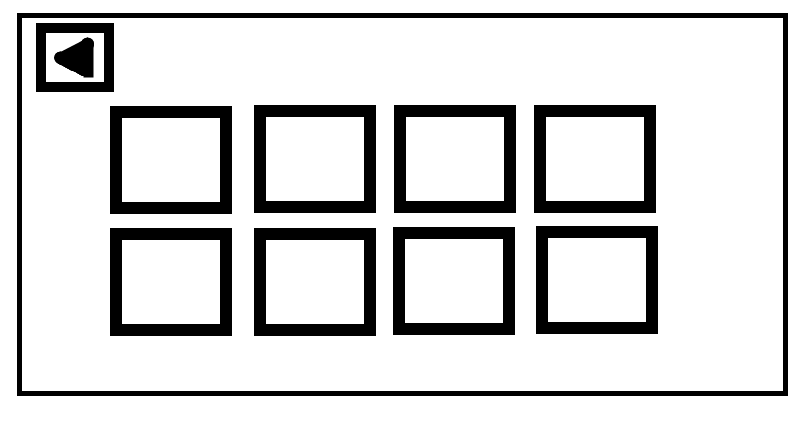
\includegraphics[width=\textwidth, height=7.5cm]{assets/Levelmenu}
	\end{minipage}
	
	\begin{minipage}{1\textwidth}
		\item \subsection*{Leveldesign:}
		Jedes Level hat den selben Grundaufbau. Am rechten Rand befindet sich eine Leiste aus der der Spieler per Drag and Drop die Spielelemente(siehe Spielaufbau) platzieren kann. Der Rest des Bildschirms nimmt das Spielfeld ein, auf dem zusätzlich am Rand Knöpfe zum Zoomen, dem aufrufen des Levelmenüs ,ansehen von Zielvorgabe und Hinweisen, sowie starten der Auswertung platziert sind.\\
		Das Levelmenü bietet die Auswahl zur Rückkehr ins Level(auswahl)menü, Hauptmenü, Neustarten des Levels und Rückkehr ins Level.\\
		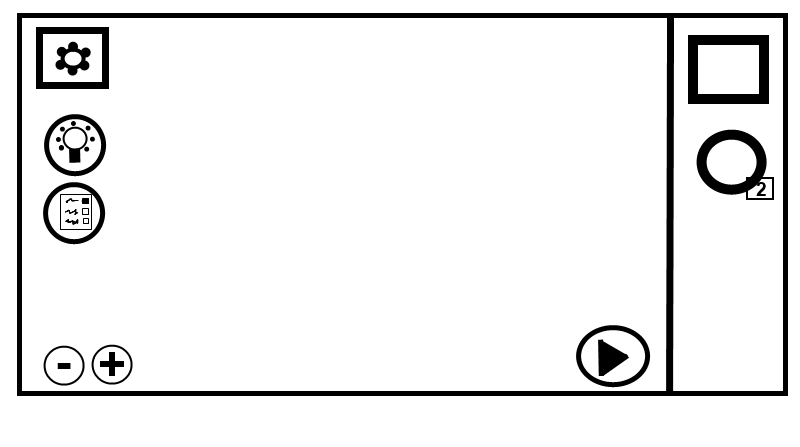
\includegraphics[width=\textwidth, height=7.5cm]{assets/LevelDesign}
	\end{minipage}
	
	\begin{minipage}{1\textwidth}
		\item \subsection*{Auswertungsmenü:}
		Hier erfährt der Spieler ob er das Level richtig gelöst hat oder nicht.
		Im Falle des Erfolgs kann der Spieler zurück zm Hauptmenü oder das nächste Level starten.
		Sollte er es nicht geschafft haben, kann er zurück zum Hauptmenü oder das Level Neustarten. Auch freigeschaltete Achievments werden hier angezeigt.\\
		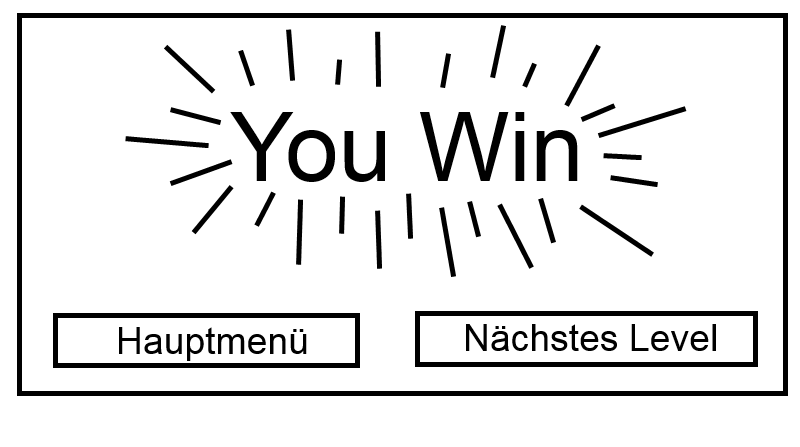
\includegraphics[width=\textwidth, height=7.5cm]{assets/Auswertungsmenu}
	\end{minipage}

\end{enumerate}

\end{document}